\documentclass[12pt]{article}
\usepackage{fullpage}
\usepackage{cite}
\usepackage{datetime}
\usepackage{geometry}
\usepackage{graphicx}
\geometry{verbose,lmargin=3cm,rmargin=3cm}

\title{Automated negotiation in the game of diplomacy - Report 3: Software Validation}
\author{Matthias Hueser, Andras Slemmer, Luca Deltodesco, Luke Tomlin, Cliff Sun}
\date{\today}

\begin{document}
\maketitle

\section{Project synopsis}
The Game of Diplomacy is a multiplayer game that removes the element of 'luck' in gameplay and replaces it with negotiation between players. 
\subsection{Aims of the project}
The over-arching goal of this project is to create an AI that is capable of negotiating with other players, whether they be human or AI, through a predefined language. This is a challenge that involves utilising many different facets of AI (learning, tactics, rationalising) and a deep understanding of the game itself.
\\
As an aside to this AI creation, we are also developing an open-source framework on which other users can build their own AIs, as well as creating a server that is capable of hosting Diplomacy games between multiple users. These are written purely in the functional programming language Haskell.
\\
By developing the frameworks and server in an open-source fashion, we are helping to develop the Diplomacy community as a whole - for instance, enabling users who are not on a Windows-based machine to play the game online or across a network. Additionally, by providing a framework for new AI creation, users are liberated from the chore of having to work at a low level and are able to simply work on the AI itself. Some users may also find the functional programming methodology more rewarding than an Obect-Oriented or Imperative approach.
\subsection{Metrics and Progress}
There are multiple ways in which we can measure the progress of our AI. Our initial milestone was to create the AI framework and the server, and then proceed to iterate a build of an AI, progressively increasing its abilities and making it better. Discussed below is how we can quantise a 'better' AI.
\subsubsection{Framework and Server progress}
It is difficult to iteratively build a server - the lowest level of operation is still quite high. There are many aspects of the Daide language to be implemented (it was quite a large language), as well as many functions related to a game of Diplomacy. Before the server can be classed as 'working', it has to adhere to a strict specification, all of which has to be supported. Fortunately some aspects of it are different from others - for instance, the connection and messaging portions can be tested seperately from the game management areas. The same goes for an AI framework - without a functional AI to plug into the framework (which doesn't exist yet) it is a challenge to know exactly if it will work as intended. Once a working version has been created, however, it is quite simple to see it improve, as new (additional) features are added and bugs ironed out.
\\
AI creation also began at the same time as the AI framework creation. This means that as new features are added to the framework, old features may no longer be supported or their implementation is changed, resulting in changes being required to the AI. However this was also beneficial in the opposite direction - as the AI gained functions and became more complicated, it became evident that additional features were required in the framework, which were then added.

\subsubsection{AI progress}
An initial set of milestones is already present on the Daide wiki. It describes an iteratively improved bot, that gains functionality and depth on each iteration. As described in an earlier report, the first bot (HoldBot) is simply an AI that works, but does nothing. After this, RandomBot is created, which gains the ability to analyse what moves are available to it, and then randomly perform one of them. As you can see, whereas HoldBot simply is 'functional', but essentially blind, RandomBot is capable of evaluating a decision (albeit possibly a bad one). After this, negotation aspects are added, further increasing the abilities of the bot itself. 
\\
Within each of these milestones, we can weigh a bot's ability using its only application - playing the game of diplomacy. For this, we need to come up with a set of metrics with which we can evaluate a players performance in a game. Some key indicators include:

\begin{itemize}
\item The number of supply depots owned at the end of the game.
\item If the player actually wins the game
\item Units lost throughout the game
\item Provinces conceded throughout the game
\end{itemize}

These are not all of the same value, of course. Winning a game is possibly the most important aspect of a game of diplomacy - if the AI somehow manages to negotiate each of the players in such an extraordinary fashion as to persuade them to surrender, it is obviously playing extremely well! 
\\
With regards to supply depots, the winning player will own half of them (eighteen), with the second-most successful player owning the second highest amount, and so on and so forth. A player with no supply-depots is very close to becoming a losing player.
\\
Units lost is a difficult metric to quantise - whilst it may immediately seem that losing many units is a bad thing, these could be due to tactical masteries involving trapping and deluding many foes. Objectively, it is probably advisable to refrain from losing units where possible.
\\
Similarly, conceding provinces, unless done in a planned fashion, is a general indicator that a player is not performing well.
\\
Because of the conceptual simplicity of a game (in that it involves taking supply depots and provinces, using equally matched units), these are about all of the indicators that exist in a game of deplomacy.  By combining these indicators in a weighted fashion (possibly with some needed calibration), we should be able to compute an accurate score of how well an particular AI is playing. Additionally, due to the quick nature of a game amongst AIs, it is not particularly difficult to run this scoring multiple times to obtain a reliable average.
\\
An interesting aside is the concept of scoring negotiation, not just general game playing. If it were possible to evaluate other players' "attitudes" towards the AI player, one might be able to deduce the competence of a bots negotiating skills. For instance, making enemies is widely regarded as a poor move, especially if those enemies are actively hostile against you. A better tactic might be to give them the illusion of friendship, whilst aligning them for a back-stabbing manouever. If we could create a way to reliably score the subtleties of negotiation between players, it might aid us in the creation of more advanced diplomising AIs.
\\
As a corollary of this, a higher-scoring AI should generally beat a lower scoring one. We can use this fact to verify that our metric is indeed working properly. 
\\
Implementation of these measurements should not be too much of an issue. All measurements (except the hypothesised negotiation scoring) can be taken serverside without any difficulty by sampling the map-definition and unit positions between turns. With regards to negotiation scoring, individual communications between players could be intercepted, but this may prove difficult to implement without breaking the current setup.

\subsubsection{Where we are currently}
Unfortunately we suffered some setbacks in the beginning with planning and evaluation of how long it would actually take us to complete the server and framework - these miscalculations have now been addressed and we are progressing with the AI creation, concurrently with the server/framework improvements. 
\\
The HoldBot and RandomBot have been written (to the current specification of the AI framework), and improved versions are in progress. Research has already been done on implementations of these improvements, so all things considered it shouldn't be particularly hard to get them up and running. Progress can now also be checked against ready-made bots from the Daide server using the metrics mentioned above.

\section{Software Validation}
\subsection{Testing}
\subsubsection{Quickcheck}
\subsubsection{Unit tests}
\subsubsection{Acceptance tests}
\subsection{General Validation}
A very practical and simple method for us to test out AI is to see if it is capable of playing with a working Daide server. Our AI framework adheres to the same language specification as Daide, so in theory should be able to play with other AIs on the server. Similarly, other AIs should be able to play on our AI server, amongst themselves and against our own AI. Of course, a 'working' AI does not necessarily mean a fully functioning one - as long as it is capable of sending the correct messages, the server will not complain. This is quite a heavy-handed approach to testing, however, as it may not always catch the niche cases.
\\
As discussed above, we can also test how well our AI is working by pitting it against other AIs. This is related to progress checks, except with a twist - we can put the AI in specific situations, where it should take a particular action, and observe its decisions. This should be easier based upon our planned implementation of move decision (in that we create a tree of facts and decisions based on these facts, with weightings. The root node (the final decision) is based upon the combination of all the decisions in the branches below), in that we can individually pick apart a decision made my the AI to see exactly why it decided to take that action.

\subsubsection{UI design testing}
There are only limited interactions with the interface on a human client. As long as the player is capable of submitting any possible move on the board (whether or not that be a valid move) and is capable of communicating with the other players, the game is classified as functioning (of course some simple window/game functions are also present, such as starting or closing a game). Then any additional features merely serve to make the user interaction easier or more pleasant.
\\
Automated testing is also a possibility, however. //BLAHBLAH STUFF HERE//

\subsubsection{Other tools}
Coding was performed in Emacs/Vim/Gedit or other similar simple text editors. No IDE was used, or code checking programs, such as lint.

\subsubsection{Code inspection}
As the AI framework was built from the ground-up, everyone in the group who wished to write or assist in writing the AI was required to know how to use the AI framework. As there is (currently) no documentation, this involved reading the written code and understanding how it worked. As such, at least two other people read a majority of the code that is written on the framework. With respect to the code of the AI, as we are at different levels of coding ability (in Haskell in particular), it has been beneficial to write the AI in pairs, so that ideas and implementations can be discussed. This is similar in many ways to Pair Programming.

\subsubsection{Stress testing}
The different aspects of our project should be stress tested in different ways. Our server for instance can be stress tested by increasing its load, for instance by sending it many messages at one time, whether they be from actual players or observers, or constructing large and elaborate orders to see if the order-resolution is capable of being completed in acceptable time. Likewise, our AI can be tested with messages as well, to see if it is capable of handling many simultaneous diplomacy messages. If it was discovered that an enemy player became less able to compute the next move if it was burdened with messages, a valid tactic might be to simply spam it with many diplomacy requests! It would be difficult to stress test the AI framework itself - its only requirement is to support the various functions for the AI, so the stress testing is most likely rolled in with the AI testing. 

\section{Managerial Documentation}
\subsection{Collaboration tools}
Collaboration has mainly been centered around GitHub, and the features present there. Resources include issue flagging, progress and milestone setting, comments and of course, code hosting. In addition to this, we have made regular use of email to schedule meetings, and discuss group progress outside of actually meeting up.

\subsection{Management/Organisational policies}
Code change and validation properties have been quite loose within the group - this is mainly due to the disparity of knowledge when it comes to how to code parts of the project. On the whole, drastic code changes have been handled either as a group or by someone with a lot more knowledge than others on the subject, and any other code changes operated on a 'trust-based' policy. Obviously, the addition of version control removes some of the risks associated with this; if someone manages to somehow delete large portions of the code, it is a simple task to restore it to a previous version.

\subsection{Knowledge transfer within the group}
As previously mentioned, there is a significant amount of knowledge variation within members of the group. Some of us are skilled with Haskell coding, whilst some of us are merely acquanted with it. Similarly, GUI design, AI design, general coding skills and other things are all varied. We have remedied this somewhat by working in pairs or more, allowing the parts of the knowledge to diffuse (in a manner similar to osmosis) between group members as problems are encountered and solved. Additionally, papers and other learning tools have been shared (via GitHub and Gmail) to aid the code writing process. Where learning-by-application and reading have failed, group members have also been keen to help each other, spending time drawing diagrams and explaining concepts.

\subsection{Group meetings}
\begin{center}
    \begin{tabular}{ | l | l | l | p{8cm} |}
    \hline
    Meeting Type       & Date          & Duration   & Summary of Meeting \\ \hline

    Supervisor         & 12/10/2011    & 1 hr       & Initial meeting with supervisor, discussing the scope of the project and confirming technologies that we were going to use. \\ \hline
    Team               & 14/10/2011    & 2 hr       & First meeting with group, discussing division of work and background reading. In addition we finalised our decision on what technologies to use and started to test compatibilities between them (Haskell and Haxe) \\ \hline
    Team               & 21/10/2011    & 2 hr       & Progress meeting to see how the server and the client were coming along. Server was to adopt the Daide protocol which provides a framework for writing a Diplomacy AI Bot and support for allowing other Daide AI Bot's to play on the server.  \\ \hline
    Team               & 28/10/2011    & 2 hr       & More progress on the server, adding ability to parsing low level daide messages and high level diplomacy messages. Client at this point is able to send commands to the server via a command line interface.  \\ \hline
    Supervisor               & 4/11/2011     & 1 hr       & Second meeting with supervisor, discussing any problems we had and how we planned to continue with building the server and the AI. In addition discussed how we would go about implementing negotation into the game.  \\ \hline

    \end{tabular}
\end{center}

\subsection{Group activity}
Due to the variation of knowledge within the group, activity has been varied and focused in different areas. 

//ELABORATION//

\subsection{Log-Book}
Our log-book records progress for the current iteration and any problems/depedancies that need to be resolved. As we have one meeting per week, in a two-week iteration we would have 3 meetings, with the first meeting being the same meeting as the final meeting of the previous iteration and the 3rd of these meetings the end-of-iteration meeting for the current iteration and the first meeting for the next iteration. The other meeting is a mid-week iteration meeting which is used to spot problems early with work possibly being distributed so that the goals of iteration can be achieved as best as possible. 
\\
At the beginning of each iteration, we plan out the work distribution that needs to be done. If more than one person is doing implementation/writing code then we need to spot any dependancies that we may have between these members (code overlapping, compatibility and overall dependancies). We make sure these dependancies are handled by making sure at each meeting whether these members of the group have sat down and made sure that they're parts would work together properly. This generally means that we often make use of pair-programming. Our logbook structure looks like something as follows:
\\ 
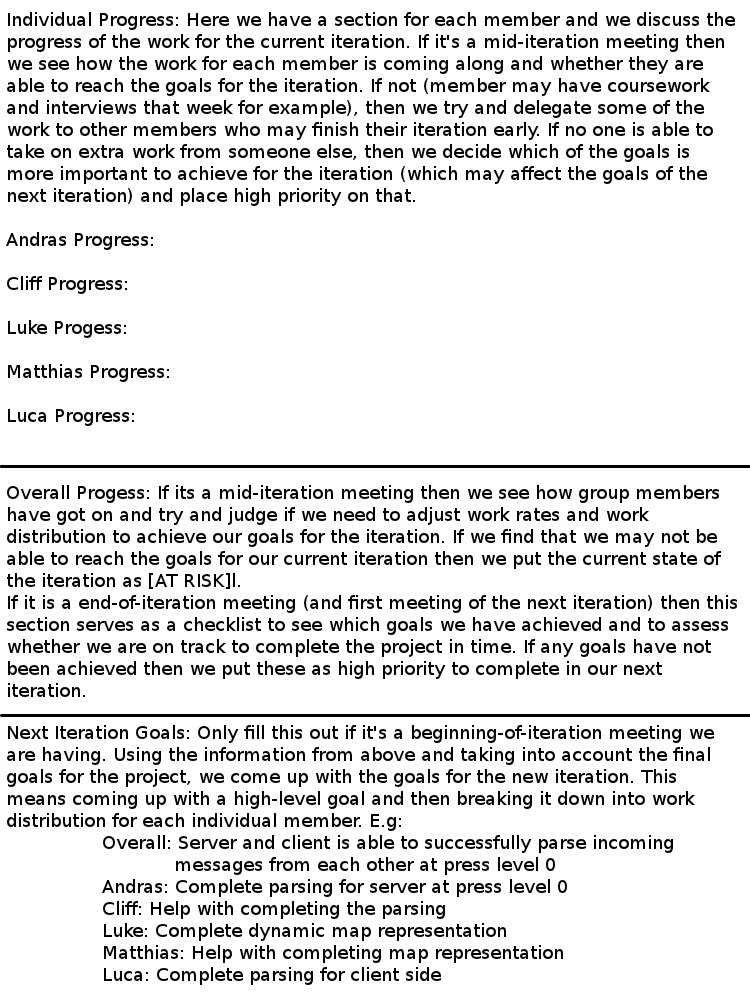
\includegraphics[width=100mm]{logbooktemplate.png}


\end{document}
